% ------------------------------------------------------------------------------
\subsection{Statistical Uncertainties on Background Rate Predictions}%
\label{app:barlow_beeston}
% ------------------------------------------------------------------------------
\subsection{Treatment of Statistical Uncertainties on Background Rate
  Predictions}%
\label{sec:barlow_beeston}

The predicted background rate in a given bin $b$ of a channel $c$ is
determined from a finite sample of events, e.g.\ from MC simulation,
and thus does not directly correspond to the true expected rate. The
background rate estimates are subject to uncertainties that have to be
considered when performing inference, particularly when bins are only
sparsely populated with events.

This uncertainty is included in the likelihood function, employing the
method proposed by Barlow and Beeston~\cite{barlow1993}, by replacing
the expected background rate from the prediction using the finite
sample with the true expected rate that has to be simultaneously
inferred. In practice this is done by performing the substitution
$\nu_{cb} \rightarrow \gamma_{cb} \nu_{cb}$ that introduces new
nuisance parameters $\gamma_{cb}$ specifying the relative difference
between the predicted and true expected rates. Initially it was
proposed to introduce one such nuisance parameter for every background
source~\cite{barlow1993}, however, a simplified version proposed in
Ref.~\cite{conway2011} is used such that only the combined uncertainty
on the total background prediction is considered instead.

The $\gamma$ nuisance parameters are constrained by auxiliary
measurements using the observed samples of events entering the
bins. These measurements contribute terms of the form
\begin{align*}
  \pois(m_{cb} | \gamma_{cb} \tau_{cb})
  \qquad \text{with} \qquad
  \tau_{cb} = \frac{( \sum_i w_i )^2}{\sum_i w_i^2} = \text{const.}
\end{align*}
to the likelihood function~\cite{cranmer2012}, where the sums go over
all events contributing to bin $b$ in channel $c$ with event weights
$w_i$. This corresponds to a measurement of the effective number of
events based on the observed value $m_{cb}$, which is nominally equal
to $\tau_{cb}$,\footnote{It should be noted that $m_{cb}$ are generally
  not integer-valued quantities and thus do not agree with the support
  of the Poisson distribution. Thus the factorial term in the Poisson
  PMF is replaced by the continuous gamma function to generalise the
  distribution to $\mathbb{R}^+$.} from the finite sample.

This approach is based on the approximation of the \emph{compound
  Poisson distribution} (CPD) that describes the distribution of the
sum of a Poisson number of random weights with a \emph{scaled Poisson
  distribution} (SPD)~\cite{Bohm:2013gla}. The CPD describes the
distribution of rate predictions based on a finite sample of weighted
events and can be defined as
\begin{align*}
  X = \sum_{i = 1}^{N} W_i \quad \text{with} \quad N \sim \pois(\lambda) \quad \text{and} \quad \text{i.i.d.\ } W_i \text{ (independent of }N\text{)} \,\text{.}
\end{align*}
It can be approximated, see for example Ref.~\cite{Bohm:2013gla},
using a scaled Poisson distribution defined by
\begin{align*}
  \tilde{X} = s \cdot \tilde{N} \quad \text{with} \quad \tilde{N} \sim \pois(\tilde{\lambda})
\end{align*}
with
\begin{align*}
  s = \frac{\expect(W^2)}{\expect(W)} \qquad \tilde{\lambda} = \frac{\lambda \expect(W)^2}{\expect(W^2)}
\end{align*}
where $\expect(W)$ and $\expect(W^2)$ are the first and second moment
of the weight distribution. The Barlow--Beeston method makes the
assumption that the expectation values can be approximated by sample
averages such that
\begin{align*}
  s = \frac{\sum_i w_i^2}{\sum_i w_i} \qquad \tilde{\lambda} = \frac{\lambda}{n} \frac{(\sum_i w_i)^2}{\sum_i w_i^2}
\end{align*}
with sample size $n$. Comparing the equation for $\tilde{\lambda}$
with the constraint term entering the likelihood function illustrates
the connection to a measurement of the effective number of events. A
number of $\tilde{N}$ events contribute with equal weights given by
$s$ to the sum, thus $\tilde{N}$ can be referred to as an effective
number of events.

These relationships will be needed in the context of the statistical
interpretation of the results in~\Cref{sec:toys_global_observables}.

%%% Local Variables:
%%% mode: latex
%%% TeX-master: "../../phd_thesis"
%%% End:



% ------------------------------------------------------------------------------
\clearpage
\subsection{Generation of Toys for the Global Significance Estimation}%
\label{app:toy_generation}
% ------------------------------------------------------------------------------
\subsubsection{Generation of Observables}

For the generation of random observables, the correlation between observables
based on the overlap of bins needs to be quantified. Let $A$ and $B$ be
observables corresponding to a pair of bins which are marginally distributed
according to Poisson distributions. The dependence between $A$ and $B$ is given
by the overlap in the kinematic region (phase space) selected by both bins. The
phase space selected by either bin can be partitioned into three parts with
associated observables $X_i$:
\begin{itemize}
\item The phase space selected by bin A but not B with observable $X_1$.
\item The phase space selected by bin A and B with observable $X_2$.
\item The phase space selected by bin B but not A with observable $X_3$.
\end{itemize}
Due to the partitioning of the phase space, the observables $X_i$ are i.i.d.\
$\pois(\lambda_i)$ with parameters $\lambda_i$ for $i = 1, 2, 3$. The
observables $A$ and $B$ can thus be written as
\begin{align*}
  A &= X_1 + X_2 \sim \pois(\lambda_1 + \lambda_2) \\
  B &= X_2 + X_3 \sim \pois(\lambda_2 + \lambda_3)
\end{align*}
and the Pearson correlation coefficient between $A$ and $B$ is given
by\footnote{$\cov(A,B) = \cov(X_1 + X_2, X_2 + X_3) = \cov(X_2, X_2) = \var(X_2)
  = \lambda_2$ from the independence of $X_1$, $X_2$, and $X_3$.}
\begin{align*}
  \rho_{AB} = \frac{\cov(A, B)}{\sqrt{\var(A)\var(B)}}
  = \frac{\lambda_2}{\sqrt{(\lambda_1 + \lambda_2) \cdot (\lambda_2 + \lambda_3)}} \,\text{.}
\end{align*}
This equation reflects the intuition that the overlap in selected phase space,
described by $\lambda_2$, induces a correlation between both observables. In the
following, the model described by $A$ and $B$ is referred to as the bivariate
Poisson model~\cite{teicher1954}.

An approximation of the correlation coefficient for all pair-wise combinations
of bins in an analysis channel can be obtained by estimating the parameters
$\lambda_i$ using MC simulation and CR data. Submatrices of the correlation
matrix obtained in the \hadhad channel are shown
in~\Cref{fig:correlation_matrix_observables}. A total of 144 bins from the
\hadhad channel enter the statistical interpretation leading to a matrix of
dimension $144 \times 144$. Similar matrices are obtained in the \lephad SLT and
LTT SRs with dimension $193 \times 193$ and $182 \times 182$, respectively.

\begin{figure}[htbp]
  \centering

  \begin{subfigure}{\textwidth}
    \centering

    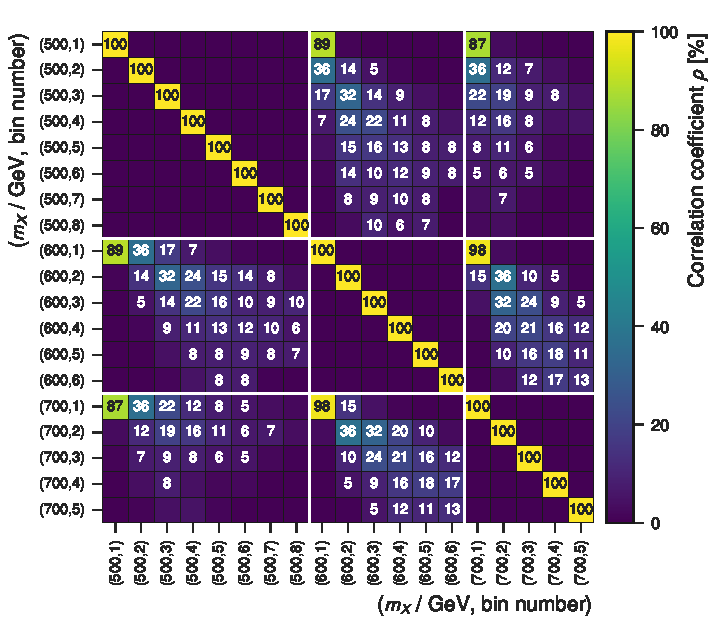
\includegraphics[scale=0.84]{global_significance/observable_correlations/corr_hadhad_medium}
    \subcaption{Submatrix for observables of the
      $\mX = 500, 600, 700\,\si{\GeV}$ discriminants}%
    \label{fig:correlation_matrix_observables_medium}
  \end{subfigure}

  \begin{subfigure}{\textwidth}
    \centering

    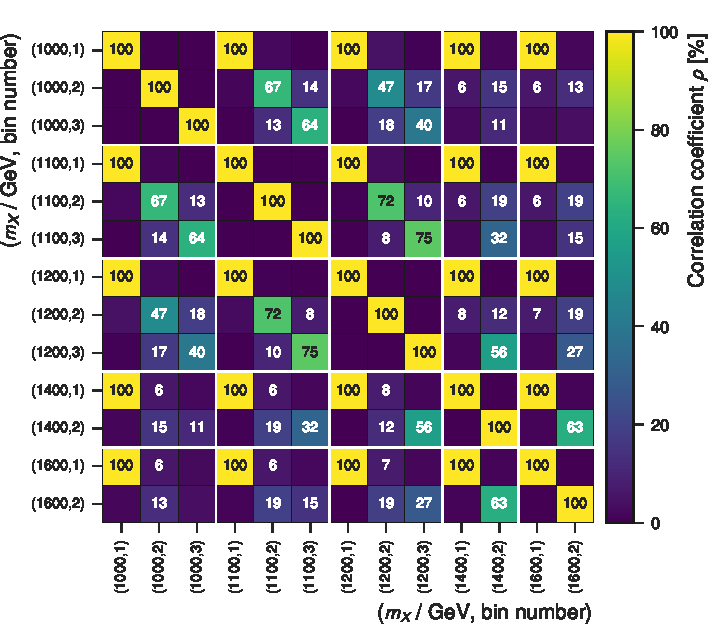
\includegraphics[scale=0.84]{global_significance/observable_correlations/corr_hadhad_high}
    \subcaption{Submatrix for observables of the
      $\mX = 1000, 1100, 1200, 1400, 1600\,\si{\GeV}$ discriminants}%
    \label{fig:correlation_matrix_observables_high}
  \end{subfigure}

  \caption{Estimate of the correlation matrix between observables of \hadhad
    channel. Two submatrices of the full matrix ($144 \times 144$) are
    shown. Bins are enumerated in ascending order of the signal probability
    according to the PNN discriminants (i.e.\ bins numbered with 1 contain the
    most background-like events for a given classification problem).  Cells are
    annotated if the correlation coefficient is larger than or equal to
    \SI{5}{\percent}. Off-diagonal elements with a correlation coefficient of
    \SI{100}{\percent} are due to rounding only.}%
  \label{fig:correlation_matrix_observables}
\end{figure}

\Cref{fig:correlation_matrix_observables_medium} shows estimated correlation
coefficients between observables of discriminants used to select signals from
resonances in the intermediate mass range in the \hadhad channel. A few features
of the correlation matrix are discussed in the following:
\begin{itemize}

\item Off-diagonal elements of submatrices describing the correlation of
  observables belonging to the same PNN discriminant are zero due to bins being
  disjoint by construction.

\item The most background-like bins (i.e.\ bins enumerated with 1) have
  correlation coefficients of about \SI{90}{\percent} or larger. This is due to
  the presence of events that are easily rejected by the PNN discriminants,
  which predominately populate the first bins. A correlation in such bins is
  expected, independent of the targeted \mX, due events being selected that are
  kinematically incompatible with resonant Higgs boson pair production. An
  example for such events are the ones where both \mMMC and \mBB are far from
  \mH.

\item The observables of the most signal-like bins are expected to have little
  correlation for the three PNN discriminants targeting the intermediate mass
  range considered in~\Cref{fig:correlation_matrix_observables_medium}.
  % The signal extraction procedure has sufficient mass
  % resolution to distinguish between signal hypotheses in the
  % intermediate mass range.
\end{itemize}

The expected correlation between observables of the high \mX discriminants are
shown in~\Cref{fig:correlation_matrix_observables_high} for the \hadhad
channel. As previously noted, the signal extraction method is unable to separate
the signatures of signal-like events at high \mX. This is reflected in the
correlation coefficient of the observables for the most signal-like bins of
adjacent mass points reaching values of up to \SI{75}{\percent}. The correlation
matrices estimated for the \lephad SLT and LTT channels yield similar results.

Considering these dependencies between observables, the toy generation for the
purpose of estimating the global significance needs to fulfil certain
requirements. First, the model needs to accurately reproduce the marginal
distributions of the observables, i.e.\ Poisson distributions with rates given
by the background estimate, such that the distribution of the discovery test
statistic for individual tests at fixed \mX can be reproduced. Second, it needs
to model the dependence structure between observables to account for the overlap
of phase space selected by the bins entering the statistical interpretation.

A multivariate extension of the bivariate Poisson distribution would fulfil
these requirements, however, such a model becomes intractable due to the large
number of observables considered, and in particular due to the presence of
negatively weighted events used for the background estimate.\footnote{In the
  absence of negatively weighted events, toy experiments could be generated
  using pseudo-data generated by drawing a random weight from $\pois(w_i)$ for
  every event with weight $w_i$ used for the background estimate. Subsequently,
  the set of pseudo-data can be used to determine the values of all
  observables. Conceptually, this approach has some parallels to resampling
  techniques like the Bootstrap
  method~\cite{10.1214/aos/1176344552,efron1994introduction}.} Instead, a model
based on the mathematical framework provided by Sklar's
theorem~\cite{Sklar1959FonctionsDR} is adopted, allowing to factorise the
marginal distributions from the dependency structure of the observables.

Sklar's theorem states~\cite{nelsen} that any $n$-dimensional joint distribution
function $H$ can be decomposed into its marginal distribution functions
$F_1, \dots, F_n$ and an $n$-dimensional copula $\mathcal{C}$. The copula
$\mathcal{C}$ is an $n$-dimensional distribution function,
$\mathcal{C}: [0, 1]^n \rightarrow [0, 1]$, with uniform marginal densities that
describes the dependencies between random variables. The joint distribution can
thus be expressed as
\begin{align*}
  H(x_1, \dots, x_n) = \mathcal{C}(F_1(x_1), \dots, F_n(x_n))
\end{align*}
according to the theorem.

For the task of generating toy experiments, the only missing piece is the
functional form of the copula since the marginal distributions are assumed to be
known from the nominal background prediction. The Poisson distribution can be
approximated by a Normal distribution provided the expected rate is not too
small, suggesting that the copula describing the dependence structure of a
multivariate Normal distribution might be applicable as an approximation. This
copula, referred to as the Gaussian copula, can be derived using the inversion
method described in Ref.~\cite{nelsen} and is given by
\begin{align}
  \label{eq:gaussian_copula}
  \mathcal{C}_{\myvec{R}}(u_1, \dots, u_n) = \Phi_{\myvec{R}}(\Phi^{-1}(u_1), \dots, \Phi^{-1}(u_n))
\end{align}
where $\Phi_{\myvec{R}}$ is the CDF of the multivariate Normal distribution with
zero mean and covariance equal to the correlation matrix~$\myvec{R}$, and
$\Phi^{-1}$ is the quantile function of the univariate Standard Normal
distribution. A review of usages of copulas for modelling multivariate count
data is given in Ref.~\cite{10.1002/wics.1398}.


The parameters $\myvec{R}$ of the Gaussian copula are estimated using the
correlation matrices derived with the bivariate Poisson model previously shown
in~\Cref{fig:correlation_matrix_observables}. The modelling assumptions are
investigated empirically in two dimensions using comparisons of simulated
results for the bivariate Poisson model and the copula-based model. The
dependence of two observables $A$ and $B$ is illustrated in
\Cref{fig:copula_model_comparison} for both models in terms of the conditional
mean and variance of $B$ given the observation $A = a$. This comparison is
performed, instead of a direct comparison of joint distribution functions, to
better illustrate the subtle differences between both models. The comparison
yields the following findings:
\begin{itemize}
\item The conditional mean of $B$ given $A = a$ agrees well between models even
  when considering bin pairs with the lowest rates $\lambda_i$ relevant for the
  analysis. This agreement is not unexpected since the Pearson correlation
  coefficient used to define the model is linked to the slope of the regression
  line that predicts $\mathrm{E}(B \vert A = a)$.

\item The conditional variance of $B$ given $A = a$ illustrates that both models
  are not equivalent, however. For bin pairs with small expected rates
  $\lambda_i$, the variance of the distribution of $B$ for fixed $A = a$ differs
  by up \SI{15}{\percent} to between both models. These deviations are assumed
  to be negligible compared to the linear trend that is properly captured by the
  model.

\item In the case of disjoint or fully overlapping\footnote{The case of fully
    overlapping bins requires special treatment since the correlation matrix
    would be singular.} bins (not shown in the figure) the bivariate Poisson
  model and copula-based model are identical.
\end{itemize}

\begin{figure}[htbp]
  \centering

  \begin{subfigure}{\textwidth}
    \centering
    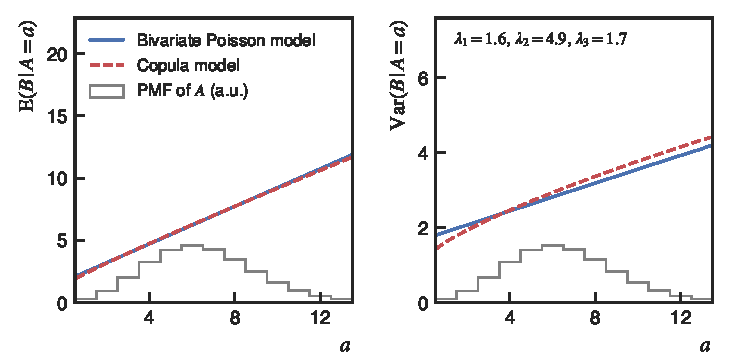
\includegraphics[scale=0.9]{global_significance/model_comparison/comparison_example_1}
    \subcaption{Most signal-like bins of the $\mX = \SI{1100}{\GeV}$
      and $\mX = \SI{1200}{\GeV}$ discriminants
      ($\rho = \SI{75}{\percent}$).}
  \end{subfigure}

  \begin{subfigure}{\textwidth}
    \centering
    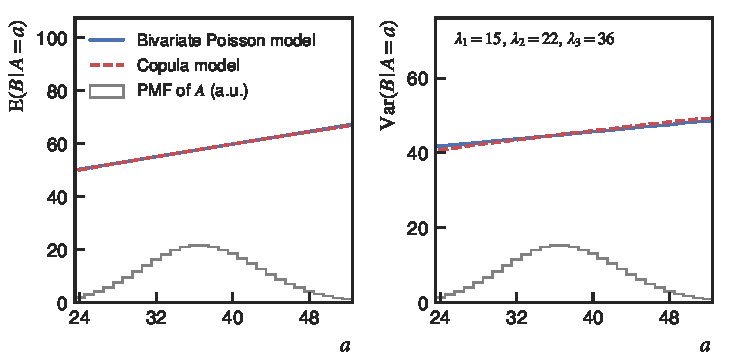
\includegraphics[scale=0.9]{global_significance/model_comparison/comparison_example_3}
    \subcaption{Second bin of the $\mX = \SI{1000}{\GeV}$ and second
      bin of the $\mX = \SI{1200}{\GeV}$ discriminant
      ($\rho = \SI{47}{\percent}$).}
  \end{subfigure}

  \begin{subfigure}{\textwidth}
    \centering
    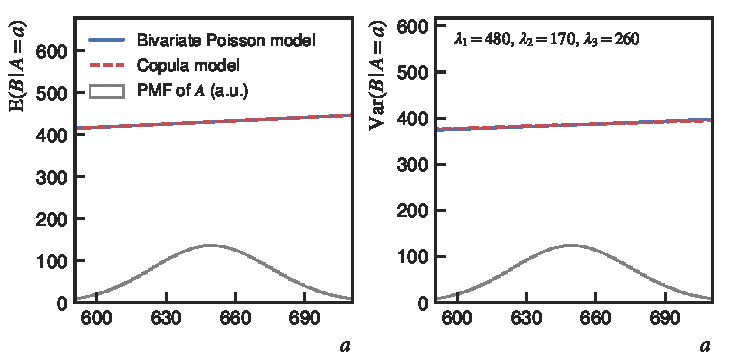
\includegraphics[scale=0.9]{global_significance/model_comparison/comparison_example_4}
    \subcaption{Third bin of the $\mX = \SI{500}{\GeV}$ and second bin
      of the $\mX = \SI{600}{\GeV}$ discriminant
      ($\rho = \SI{32}{\percent}$).}
  \end{subfigure}

  \caption{Comparison of the bivariate Poisson model and the copula model with a
    Gaussian copula specified by
    $\rho = \lambda_2 / \sqrt{(\lambda_1 + \lambda_2) \cdot (\lambda_2 +
      \lambda_3)}$ and marginal distributions given by
    $A \sim \pois(\lambda_1 + \lambda_2)$ and
    $B \sim \pois(\lambda_2 + \lambda_3)$. The conditional mean (left panels)
    and variance (right panels) of $B$ given the observation $A = a$ is shown to
    illustrate the dependence of both random variables. Three different
    scenarios are shown varying in the expected rates $\lambda_i$ and in the
    correlation coefficients $\rho$ between $A$ and $B$. The scenarios are
    chosen from bin pairs for the \hadhad channel discriminants.  The
    probability mass function (PMF) of $A$ is overlayed in arbitrary units
    (a.u.).}%
  \label{fig:copula_model_comparison}
\end{figure}

With these simplifying modelling assumptions, observables can be randomly
generated using the multivariate copula-based model. The following algorithm
allows to draw the vector of random variates $\myvec{x} = (x_1, \dots, x_n)$
from the joint distribution described by the Gaussian copula and marginal
distributions:
\begin{enumerate}
\item Draw a vector of random variates, $\myvec{u} = (u_1, \dots, u_n)$, from
  the distribution described by $\mathcal{C}_{\myvec{R}}$.

  The vector $\myvec{u}$ is obtained by generating random variates
  $\myvec{n} = (n_1, \dots, n_n)$ from the centred multivariate Normal
  distribution with covariance matrix equal to $\myvec{R}$, followed by an
  element-wise application of the univariate Standard Normal CDF to $\myvec{n}$,
  i.e.\ $u_i = \Phi(n_i)$ for every $i = 1, \dots, n$. This procedure follows
  directly from the form of the Gaussian copula in~\Cref{eq:gaussian_copula}.

  In practice, the matrices $\myvec{R}$ that are considered here are singular
  due to multicollinearity between observables. This arises from 19 implicit
  constraints due to the requirement that the sum of observables is the same for
  all 20 discriminants in a given analysis channel, thus leading to 19 vanishing
  eigenvalues of $\myvec{R}$. Therefore, multivariate Normal random variates are
  generated in a lower dimensional space that removes the collinearity, followed
  by a back-transformation to the $n$-dimensional space. The required
  transformations are provided by singular value decomposition of $\myvec{R}$.

\item Obtain $\myvec{x}$ by evaluating the quantile functions of the $n$
  marginal distributions at the values of $\myvec{u}$ from the previous step
  such that $x_i = F_{i}^{-1}(u_i)$ for $i = 1, \dots, n$. The marginal
  distribution functions are given by Poisson distributions with expected rates
  corresponding to the background prediction in a given bin.
\end{enumerate}
The multivariate count data generated with this method was inspected by
generating large samples of size $\mathcal{O}(10^6)$ showing agreement in terms
of the expected marginal distributions of the observables and closely
reproducing the pair-wise correlation coefficients estimated with the bivariate
Poisson model.


\subsubsection{Generation of Global Observables}

Global observables have to be fluctuated when estimating the global significance
with toy experiments. This section will focus on the generation of the global
observables related to the Barlow--Beeston method, previously described in
\Cref{app:barlow_beeston}, that is used to include statistical uncertainties on
the predicted background rates in the likelihood function. Due to the
statistical nature of these uncertainties they cannot be neglected when
estimating the global significances, particularly since these uncertainties have
a large impact on the POI.

Global observables related to all other systematic uncertainties are randomly
assigned given their constraint terms in the likelihood function and assumed to
be fully correlated between all tests. A detailed discussion of these is omitted
since standard procedures are used.

Regarding global observables associated with the Barlow--Beeston method, similar
considerations can be made as for the observables discussed in the previous
section. The phase space selected by pairs of bins can partially overlap,
leading to dependencies between the background rate predictions (from simulation
and CR data) between bins. The random generation of these (global) observables
is simplified, however, since resampling methods can be used.

The sample of simulated and CR events used to predict the background rates in
all bins of the discriminants can be resampled using non-parametric Bootstrap
methods~\cite{10.1214/aos/1176344552,efron1994introduction} to obtain replicas
of the sample that capture the statistical uncertainties and correlations
between background rate predictions. Every event in the original sample is
assigned a random bootstrap weight $w_i^{\text{b}}$ drawn from
$\pois(\lambda = 1)$ serving as an approximation to the regular non-parametric
Bootstrap~\cite{google:poisson,ATL-PHYS-PUB-2021-011}. The resulting bootstrap
replica provides new rate estimates for all bins given
by~$\sum_{i} w_{i}^{\text{b}} w_i$, where $w_i$ is the nominal event weight,
$w_i^{\text{b}}$ the bootstrap weight, and the sum goes over all events falling
into bin $b$ of channel $c$. These rate estimates can be translated into the
observed effective number of events $m_{cb}$ (global observables of the
Barlow--Beeston method) using
\begin{align*}
  m_{cb} = \frac{1}{s_{cb}} \sum_{i} w_{i}^{\text{b}} \, w_i
\end{align*}
with the scaling factor given by $s_{cb} = \sum_i w_i^2 / \sum_i w_i$, and sums
going over all events falling into bin $b$ of channel $c$. This relationship
follows from the scaled Poisson approximation employed by the Barlow--Beeston
method introduced in~\Cref{app:barlow_beeston}. Multiple toy experiments are
generated by repeating the Bootstrap procedure.

In~\Cref{fig:comparison_bootstrap_poisson} the distributions of two exemplary
global observables in the \hadhad channel are shown and compared with the
distribution used to define the auxiliary measurement in the likelihood
function. In general, both are not expected to agree perfectly due to the
approximations used by the Barlow--Beeston method, however, both approaches agree
well for scenarios relevant to this analysis. Even in the case depicted
in~\Cref{fig:comparison_bootstrap_poisson_lowest_tau}, which corresponds to the
bin with the smallest effective number of events of the \hadhad channel (in part
due to large fraction of negatively weighted events), the agreement between both
methods is sufficient.

\begin{figure}[htbp]
  \centering

  \begin{subfigure}{0.485\textwidth}
    \centering

    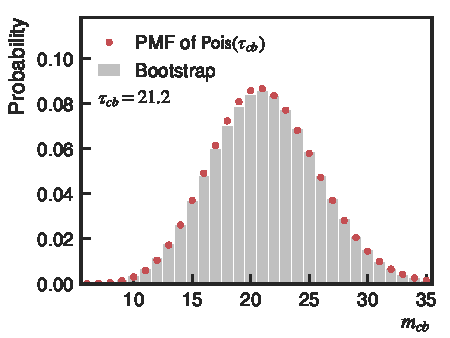
\includegraphics[width=0.98\textwidth]{global_significance/gamma_globs/gamma_obs_251}
    \subcaption{Most signal-like bin of the $\mX = \SI{251}{\GeV}$
      discriminant in the \hadhad-channel.}%
    \label{fig:comparison_bootstrap_poisson_lowest_tau}
  \end{subfigure}\hfill%
  \begin{subfigure}{0.485\textwidth}
    \centering

    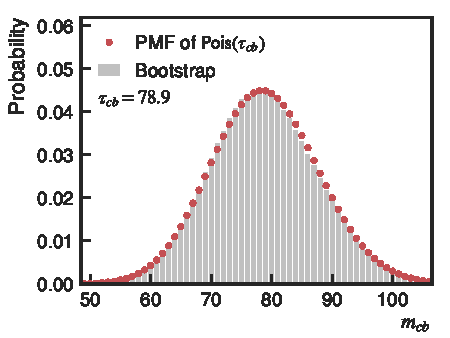
\includegraphics[width=0.98\textwidth]{global_significance/gamma_globs/gamma_obs_1000}
    \subcaption{Most signal-like bin of the $\mX = \SI{1000}{\GeV}$
      discriminant in the \hadhad-channel.}
  \end{subfigure}

  \caption{Comparison of marginal distributions of global observables from the
    Barlow--Beeston method. The red markers show the Poisson distribution used to
    define the constraints on the $\gamma_{cb}$ NPs ($\gamma_{cb} = 1$ is
    assumed) in the likelihood function. The grey histogram shows the
    distribution of the global observable following the Bootstrap approach that
    accounts for correlations of $m_{cb}$ between bins. Statistical
    uncertainties on the Bootstrap histogram are negligible.}
  \label{fig:comparison_bootstrap_poisson}
\end{figure}


%%% Local Variables:
%%% mode: latex
%%% TeX-master: "../../phd_thesis"
%%% End:



% ------------------------------------------------------------------------------
\clearpage
\subsection{Breakdown}%
\label{app:breakdown_table}
% ------------------------------------------------------------------------------

\begin{table}[htbp]
  \centering

  \caption{Decomposition of the variance on $\hat{\sigma}$, the
    maximum likelihood estimate of the cross section
    $\sigma(pp \to X\to HH)$, by uncertainty category for the fit to
    Asimov data with $\mu = 0$ in all regions. The decomposition is
    determined analogously to~\Cref{tab:breakdown_nonres}, separately
    for four exemplary signal mass hypotheses. The fractions of
    subcategories do not necessarily sum to the fraction of the parent
    category due to correlations between nuisance parameters.}%
  \label{tab:breakdown_res_exp_mu0}

  \begin{tabular}{
  l
  S[table-format=2.0, table-space-text-pre=\textless, table-column-width=1.6cm]
  S[table-format=2.0, table-space-text-pre=\textless, table-column-width=1.6cm]
  S[table-format=2.0, table-space-text-pre=\textless, table-column-width=1.6cm]
  S[table-format=2.0, table-space-text-pre=\textless, table-column-width=1.6cm]
  }
  \toprule
         & \multicolumn{4}{c}{Explained fraction of variance on $\hat{\sigma}$}\\
         %& \multicolumn{4}{c}{of variance on $\hat{\mu}$}\\
  \cmidrule{2-5}
  Source & {$\SI{300}{\GeV}$} & {$\SI{500}{\GeV}$} & {$\SI{1000}{\GeV}$} & {$\SI{1600}{\GeV}$} \\
  \midrule
  \textbf{Data statistical uncertainty}
         & 59\,\si{\percent} & 81\,\si{\percent} & 82\,\si{\percent} & 82\,\si{\percent} \\
  \textbf{Systematic uncertainties}
         & 41\,\si{\percent} & 19\,\si{\percent} & 18\,\si{\percent} & 17\,\si{\percent} \\
  \hspace{0.8em} Instrumental uncertainties
         & 10\,\si{\percent} & 1\,\si{\percent} & 1\,\si{\percent} & {\textless} 1\,\si{\percent}\\
  \hspace{0.8em} Signal modelling uncertainties
         & 1\,\si{\percent}  & 1\,\si{\percent} & {\textless} 1\,\si{\percent} & 3\,\si{\percent} \\
  \hspace{0.8em} Background statistical uncertainties
         & 18\,\si{\percent} & 11\,\si{\percent} & 7\,\si{\percent} & 9\,\si{\percent} \\
  \hspace{0.8em} Background modelling uncertainties
         & 12\,\si{\percent} & 7\,\si{\percent} & 10\,\si{\percent} & 5\,\si{\percent} \\
  \midrule
  \hspace{1.6em} -- \hspace{0.2em} Top-quark (incl.\ free normalisation)
         & 3\,\si{\percent} & 2\,\si{\percent} & 1\,\si{\percent} & {\textless} 1\,\si{\percent} \\
  \hspace{1.6em} -- \hspace{0.2em} \ZHF (incl.\ free normalisation)
         & 3\,\si{\percent} & 1\,\si{\percent} & 3\,\si{\percent} & 2\,\si{\percent} \\
  \hspace{1.6em} -- \hspace{0.2em} SM Higgs boson
         & {\textless} 1\,\si{\percent} & 2\,\si{\percent} & 3\,\si{\percent} & 2\,\si{\percent} \\
  \hspace{1.6em} -- \hspace{0.2em} Fake-\tauhadvis
         & 4\,\si{\percent} & {\textless} 1\,\si{\percent} & 1\,\si{\percent} & 1\,\si{\percent} \\
  \hspace{1.6em} -- \hspace{0.2em} Other
         & {\textless} 1\,\si{\percent} & {\textless} 1\,\si{\percent} & {\textless} 1\,\si{\percent} & {\textless} 1\,\si{\percent} \\
  \bottomrule
\end{tabular}

%%% Local Variables:
%%% mode: latex
%%% TeX-master: "../phd_thesis"
%%% End:

\end{table}


% ------------------------------------------------------------------------------
\clearpage
\subsection{Pulls/Rankings Resonant?}%
\label{app:rankings_resonant}
% ------------------------------------------------------------------------------

\todo[inline]{Add for 3 examples: 300, 500, 1000.}


%%% Local Variables:
%%% mode: latex
%%% TeX-master: "../../phd_thesis"
%%% End:
